\icode{E-MD-SI-L3-261115-002}
如图所示，$A$、$B$、$C$三球的质量均为 $m$，轻质弹簧一端固定在斜面顶端、另一端与 $A$ 球相连，$A$、$B$ 间固定一个轻杆，$B$、$C$ 由一轻质细线连接。倾角为 $\theta$ 的光滑斜面固定在地面上，弹簧、轻杆与细线均平行于斜面，初始时系统处于静止状态，细线被烧断的瞬间，下列说法不正确的是\paren[]
	
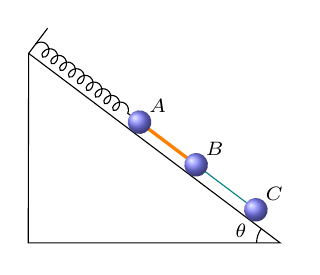
\begin{tikzpicture}[font=\scriptsize]
	\begin{scope}[rotate=-37]
		\draw (-4,.4)--(-4,0)--(0,0)--++(-143:3.2)--(-4,0);
		\draw[decoration={aspect=.8,segment length=4,amplitude=.8mm,coil},decorate] (-4,.15)--(-2.5,.15);
		\draw[teal] (-1.45,.15)--(-.5,.15);
		\draw[very thick,orange] (-2.35,.15)--(-1.45,.15);
		\foreach \x/\c in {-2.35/A,-1.45/B,-.5/C}
			\shade[ball color=blue!50] (\x,.15)node[above right]{\(\c\)} circle(.15);
	\end{scope}
	\draw (-.3,0) arc(180:143:.3);
	\node at(-.5,.15){\(\theta\)};
\end{tikzpicture}
\begin{choices}
	\item $B$ 球的受力情况未变，加速度为零
	\item $A$、$B$ 两个小球的加速度均沿斜面向上，大小均为 $\frac{1}{2}g\sin\theta$
	\item $A$、$B$ 之间杆的拉力大小为 $\frac{3}{2}mg\sin\theta$
	\item $C$ 球的加速度沿斜面向下，大小为 $g\sin\theta$
\end{choices}
\begin{answer}
    A\qquad 提示：
\end{answer}